
\section{Multivariate analysis}
\label{sec:mva}

After the traditional cut-based analysis presented in the previous section,
and combining the significance of the different event categories,
we end up with a $S/\sqrt{B}$ value around $1.2$.
%
This is not enough to claim observation in this channel.
%
however, the attentive reader might have noticed that we have used
relatively 
loose kinematics cuts, for example in the Higgs mass window.
%
The motivation for this is that the $n$-tuples of signal and background
events, after our basic selection, are processed though a multivariate
analysis with the motivation to increase the signal over background
significance.
%
Multivariate techniques are by now a common tool to enhance signal
significance in HEP analysis, and rightly so,
since they open a new window to improve the performance
of many physics analysis and searches.
%
For instance, the UCL $hh\to 4b$ analysis~\cite{Wardrope:2014kya}
uses a Boosted
Decision Tree MVA to improve signal discrimination.

\subsection{MVA strategy: deep neural networks}

The classification of events as arising from either signal or
background processes via the use of a multivariate analysis is a common
technique in high energy physics~\cite{Baldi:2014pta,Wardrope:2014kya}.
%
In our work we use a specific type of  MVA to
disentangle signal and background events in the $hh\to 4b$ process,
in particular we use a feed-forward artificial neural network (ANN).
%
The basic idea is that the ANN is given both all MC signal and background
events which satisfy the basic selection cuts {\bf C1}, allowing to identify
which are the most relevant variables to discriminate between the two.

In this work, the ANN that we use has the following architecture.
\be
\label{eq:nn1}
N_{\mathrm{var}}\times5\times3\times1 \, ,
\ee
where $N_{\mathrm{var}}$ represents the number of input variables for the MVA.
All neural-network layers use a sigmoid activation function, allowing
for a probabilistic
interpretation of the neural-network output, including in the final layer.
%
In Fig.~\ref{fig:nnarch} we show an example of the ANN that we use in this work, corresponding here
to the case of the resolved category.

%%%%%%%%%%%%%%%%%%%%%%%%
\begin{figure}[t]
  \begin{center}
      \vspace{-1cm}
  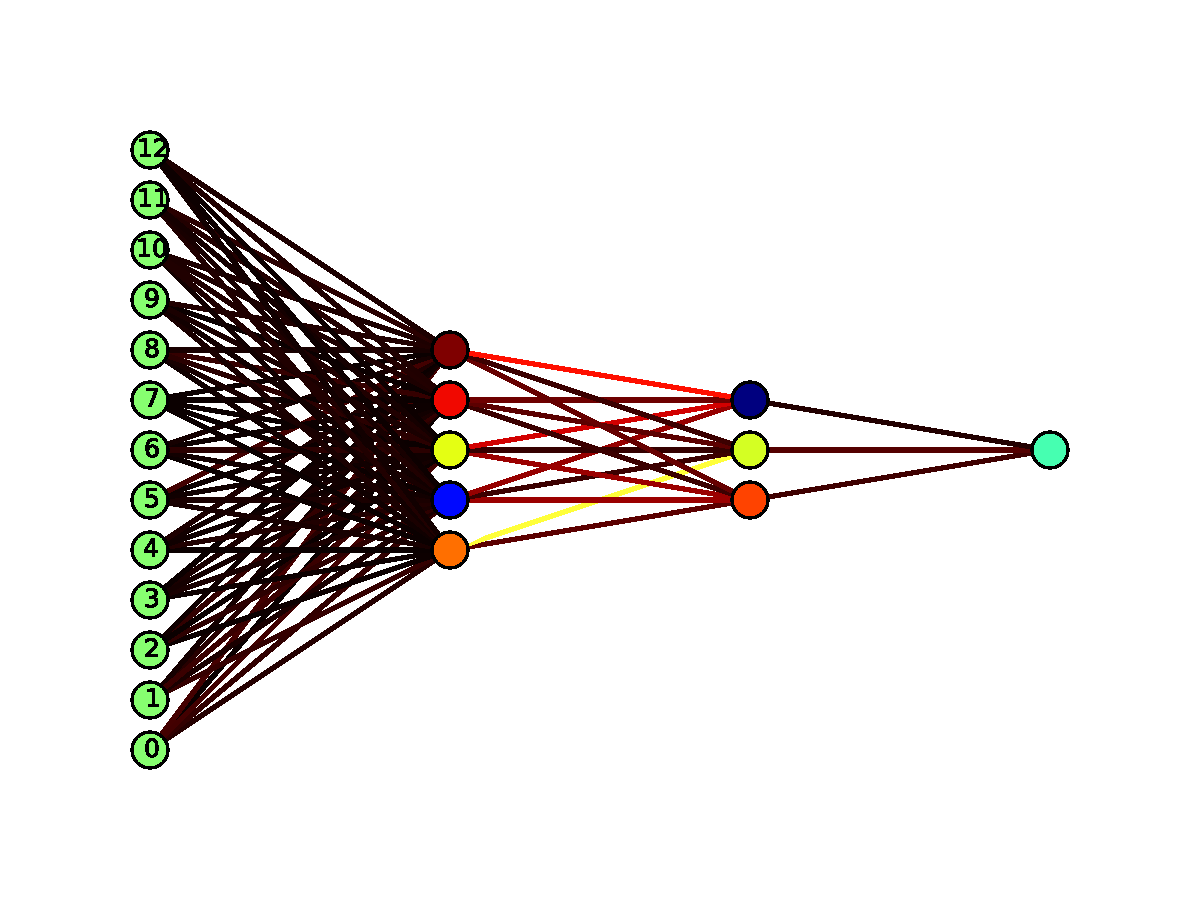
\includegraphics[width=0.80\textwidth]{plots/res_nnarch.pdf}
  \vspace{-1cm}
\caption{\small Architecture of the ANN used for the analysis of the resolved
  category, with $N_{\rm var}=13$ input variables and thus the same number of neurons
in the first layer.}
\label{fig:nnarch}
\end{center}
\end{figure}
%%%%%%%%%%%%%%%%%%%%%%%

The training of the ANN for the signal/background classification task
proceeds as follows.
%
Given a set of $N_{\mathrm{var}}$  kinematic variables $\{k\}_i$ associated with the event $i$, and a set of neural network parameters $\{\omega\}$, we interpret the neural network output $y_i$ (that is, the activation state of the
neuron in the last layer)
as the probability that the event $i$ originates from the signal process,
\be
y_i = P(y^\prime_i=1|\{k\}_i, \{\omega\} )\, ,
\ee
where $y_i^\prime$ represents the true classification of the event $i$, i.e $y^\prime_{\text{signal}} = 1$ and $y^\prime_{\text{background}} = 0$. With this interpretation, our general classification probability including background events is given by
\be
P(y_i^\prime|\{k\}_i, \{\omega\}) = y_i^{y^\prime_i}(1-y_i)^{1-y^\prime_i} \, ,
\ee
which implies that the  negative log-likelihood cost function
that needs to be minimized during the ANN training is 
the cross-entropy error, defined as
 \bea
 E(\{\omega\}) &=& -\log\left(\prod_i^{N_{\text{evt}}} P(y_i^\prime|\{k\}_i, \{\omega\})\right)\nonumber\\
 &=&
 \sum_i^{N_{\text{evt}}} y^\prime_i\log{y_i} + (1-y^\prime_i)\log{(1-y_i)} \, ,
 \label{cross-entropy}
 \eea
 where $N_{\text{evt}}$ is the number of
 Monte Carlo events that we have generated.
 %
 The ANN is trained both on the signal and background MC events,
 in each case using the information $y_i'$ of the true nature
 of the event.
 %
 To be stable against statistical fluctuations, it is important to use
 a large enough MC sample both of signal and of background events
 for the MVA training.
 
 Therefore, the training of the neural networks consist on the
 minimization of the cross-entropy error,
 Eq.~\ref{cross-entropy}, which in this work is achieved using a
 Genetic Algorithm.
 %
 Since given the large number of events the probability of
 over-fitting is tiny, we just train the MVA for a very long
 number of generations, in this case $N_{\rm gen}=50k$.
 %
 We have verified that if a larger number of generations
 are used the results are unchanged.
 %
 We have also verified that using a cross-validation stopping
 criterion as in the NNPDF3.0 fits does not affect the results.

 

 \subsection{Input kinematical variables for the MVA}
 \label{sec:input}

 To identify the most discriminatory variables, we have to train
 the MVA using a large number of kinematic distributions for
 signal and background events.
%
In our $hh\to 4b$ case,
the input variables for the MVA differ between our three categories,
since in the case of large-$R$ jet reconstruction we want to exploit
the richness of substructure information.

For the three categories, boosted, intermediate and resolved,
the following common variables are used as input to the MVA:
\begin{itemize}
\item The transverse momenta of the leading and subleading Higgs, $p_{T,h_1}$ and $p_{T,h_2}$.
\item The transverse momentum of the reconstructed Higgs pair, $p_{T,hh}$
\item The invariant masses of the leading and sub-leading Higgs candidates, $m_{h,1}$ and $m_{h,2}$.
\item The invariant mass of the reconstructed Higgs pair, $m_{hh}$.
\item The separation in $R$ between the two Higgs candidates, $\Delta R_{hh}$.
\item The separation in $\phi$  between the two Higgs candidates, $\Delta \phi_{hh}$.
\item The separation in $\eta$  between the two Higgs candidates, $\Delta \eta_{hh}$.
\item In the boosted category,
  the transverse momenta of the leading, $p_{T,h_{1,1}}$ and $p_{T,h_{1,2}}$ and
  sub-leading, $p_{T,h_{2,1}}$ and $p_{T,h_{2,1}}$, Higgs candidate subjets.
  %
  In the resolved category instead, we use the transverse momenta $p_{T,i}$ of the four leading 
   $b$-tagged small-$R$ jets in the event. 
\end{itemize}
Therefore, we have a total of 13 variables which are common to the three categories.
%


For analyses involving the use of large-$R$ jets,
namely for the boosted and intermediate categories,
a number of jet substructure variables~\cite{Aad:2013gja} is used
for every large-$R$ jet that is used for the Higgs reconstruction.
%
In particular we include in the MVA training for each large-$R$ jet
\begin{itemize}
\item The $k_T$ splitting scale~\cite{Butterworth:2002tt,Butterworth:2008iy}.

  This variable is defined by reclustering the constituents of a jet with the
  $k_t$ algorithm, which usually clusters last the harder constituents, and then
  taking the $k_t$ distance measure between the two subjets at the final stage of the recombination
  \be
\sqrt{d_{12}} \equiv {\rm min}\lp p_{T,1},p_{T,2}\rp \cdot \Delta R_{12} \, ,
\ee
where one can also define related variables like $\sqrt{d_{23}}$ that corresponds to the
splitting scale in the second-to-last clustering.
  
\item The ratio of 2-to-1-Subjetiness $\tau_{12}$~\cite{Thaler:2010tr,Thaler:2011gf}.

  The $N$-subjettiness variables $\tau_N$ are defined by clustering the constituents
  of a jet with the exclusive $k_t$ algorithm and requiring that $N$ subjets are found,
  \be
  \tau_N \equiv \frac{1}{d_0} \sum_k p_{T,k}\cdot {\rm min}\lp \delta R_{1k}, \ldots,
  \delta R_{Nk}\rp \, , \qquad d_0\equiv \sum_k p_{T,k}\cdot R \, ,
  \ee
  with $ p_{T,k}$ the $p_T$ of the constituent $k$ and $\delta R_{ik}$ the distance from
  subjet $i$ to constituent $k$.
  %
  In this work in particular we use as input to the MVA
  \be
\tau_{21} \equiv \frac{\tau_2}{\tau_1} \, ,
  \ee
  which provide good discrimination between QCD jets and jets arising from the decay of
  a heavy resonance.
  
\item The energy correlation function double-ratios $C_2$ and $D_2$~\cite{Larkoski:2013eya}.

  The energy correlation double ratio $C_2$ is defined
  as
  \be
C_2^{\beta} \equiv \frac{ {\rm ECF}(3,\beta) {\rm ECF}(1,\beta)}{{\rm ECF}(2,\beta)} \, ,
  \ee
  where the energy correlation functions ${\rm ECF}(3,\beta)$ are defined
  in~\cite{Larkoski:2013eya} with the motivation that $(N+1)$-point correlators
  are sensitive to $N$-prong substructure.

\end{itemize}
%
Therefore, there are in total $N_{\mathrm{var}}=13$ variables for the resolved analysis,
17 for the semi-resolved, and 21 for the boosted category.
%
Given that the MVA is able to identify the most discriminatory variables
and to ignore those that have smaller effect, it is advantageous to
include as many substructure variables as possible.
%
As we will show, the use of substructure variables in the MVA is the key to increase the signal
significance in the boosted category.

\subsection{Enhancing signal discrimination with MVA}

Let us now present the results of the MVA applied to the event samples
that satisfy the cut-based analysis discussed in the previous section.
%
First of all in Fig.~\ref{fig:nnresponse} we show the distribution of
the ANN output, after the training for signal and background events, for the three
exclusive categories.
%
All distributions have been normalized, so that their integral
  adds up to one.
%
Given that the final separation between signal and background will be achieving by introducing
a cut in the ANN output, the more separated that the two distributions are, the more efficient
the MVA discrimination will be.



%%%%%%%%%%%%%%%%%%%%%%%%%%%%
\begin{figure}[t]
\begin{center}
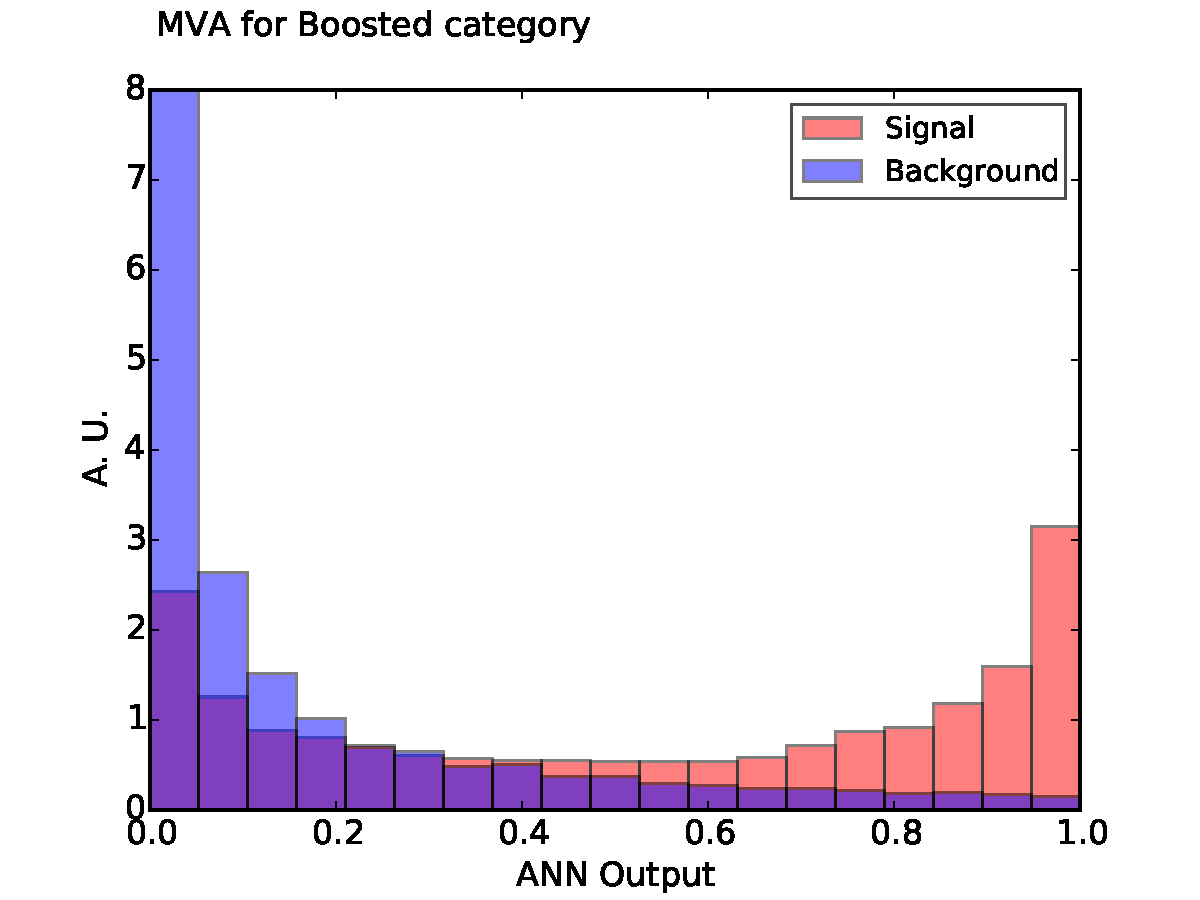
\includegraphics[width=0.65\textwidth]{plots/Boosted_disc.pdf}
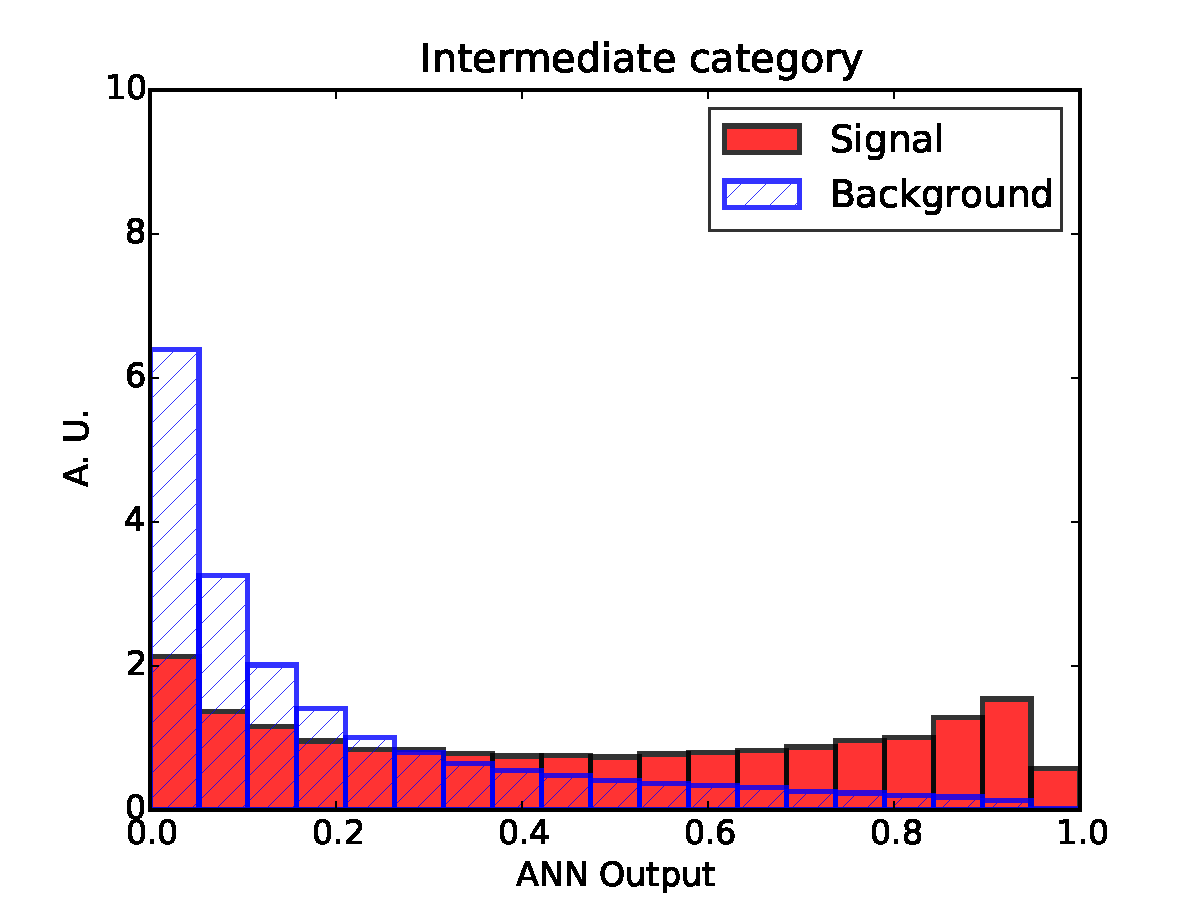
\includegraphics[width=0.48\textwidth]{plots/Intermediate_disc.pdf}
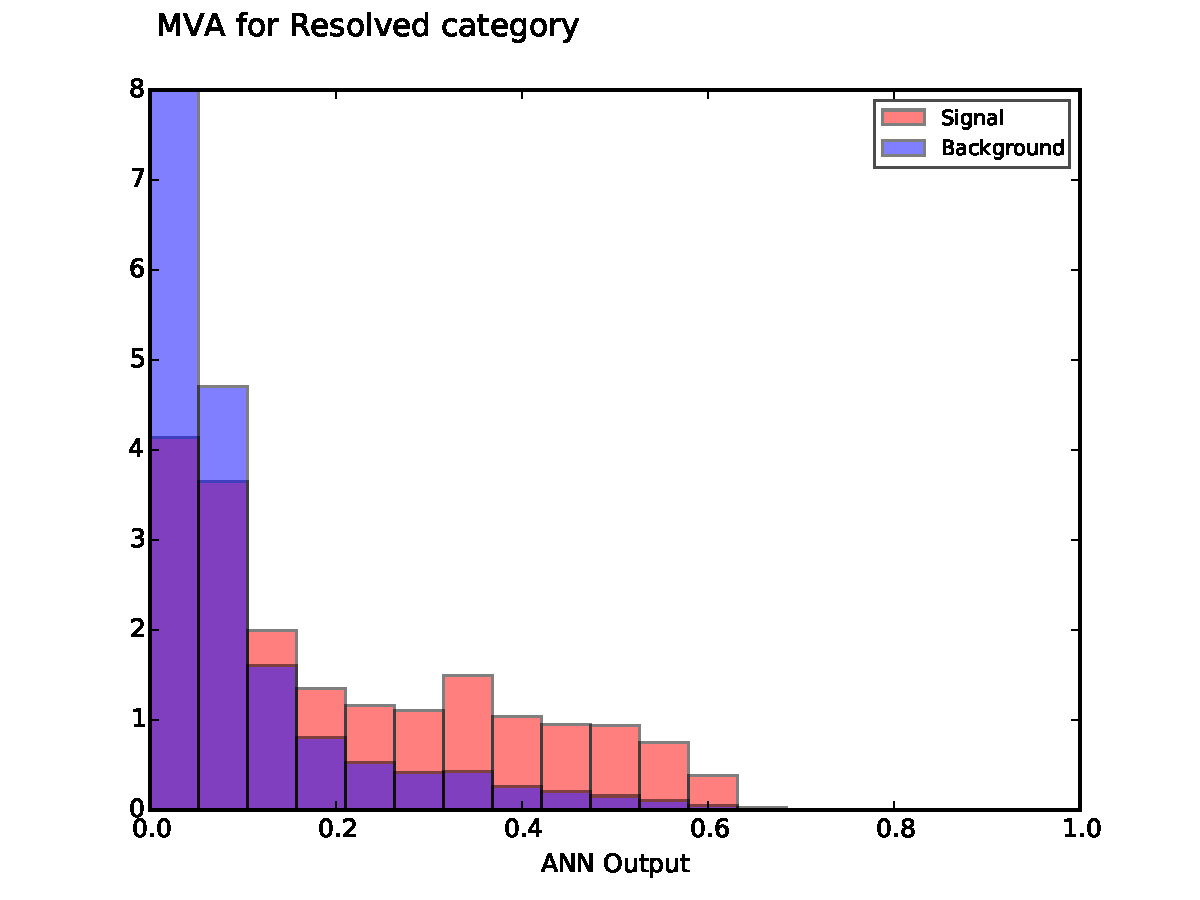
\includegraphics[width=0.48\textwidth]{plots/Resolved_disc.pdf}
\caption{\small The distribution as a function of the ANN output
  for the signal and background MC events in the three categories:
  boosted (upper plot), intermediate (lower left plot) and
  resolved (lower right plot).
  %
  All distributions are normalized so that their integral
  adds up to one.
}
\label{fig:nnresponse}
\end{center}
\end{figure}
%%%%%%%%%%%%%%%%%%%%%%%

From Fig.~\ref{fig:nnresponse} we see that in the boosted category the MVA manages
to achieve a clear discrimination between signal and background, with the two distributions
nicely peaking at 1 and at 0 respectively.
%
This indicates that introducing a suitable cut in the ANN output will substantially reduce the background,
while keeping a reasonable signal efficiency.
%
The performance of the MVA discrimination is similar though slightly worse in the intermediate
category, and it is markedly worse in the resolved category.
%
We have traced back these differences to the use of jet substructure variables
in the boosted and intermediate categories, which induce the maximum
discrimination between signal and background events.



The results for the signal selection efficiency and the 
background rejection rate as a function of the cut in the ANN output
define the so-called  Receiver-Operating Characteristic (ROC)
curve.
%
It is clear that we can achieve a very high signal efficiency by using
a small value of the cut in the ANN output, but this choice will be
affected from a poor background
rejection.
%
Conversely, using a higher value of the cut will increase background rejection at the
cost of dropping signal efficiency.
%
The usefulness of ROC curves is that they allow to determine the
optimal cut value that removes enough background without degrading too much the signal efficiency.
%
In addition, it is important to select a value of the cut in ANN output so that
the number of expected signal events is still large enough.


In Fig.~\ref{fig:exampleroc} the
we show the ROC curve for the background rejection rate as a function of the signal
  selection efficiency as the cut in the ANN output is varied.
  %
  We show the results for the three exclusive categories: boosted, intermediate
  and resolved.
%
As could already be inferred from the distribution of neural
networks output in Fig.~\ref{fig:nnresponse}, we find
that the neural network MVA is reasonably efficient
in discriminating signal over background.
%
The performance is best in the case of the boosted category,
decreasing then for the intermediate and finally for the
resolved categories, consistent with the distributions in
Fig.~\ref{fig:exampleroc}.
%



%%%%%%%%%%%%%%%%%%%%%%%%%%%%%%%%%%%%%%%%%%%%%%
\begin{figure}[t]
\begin{center}
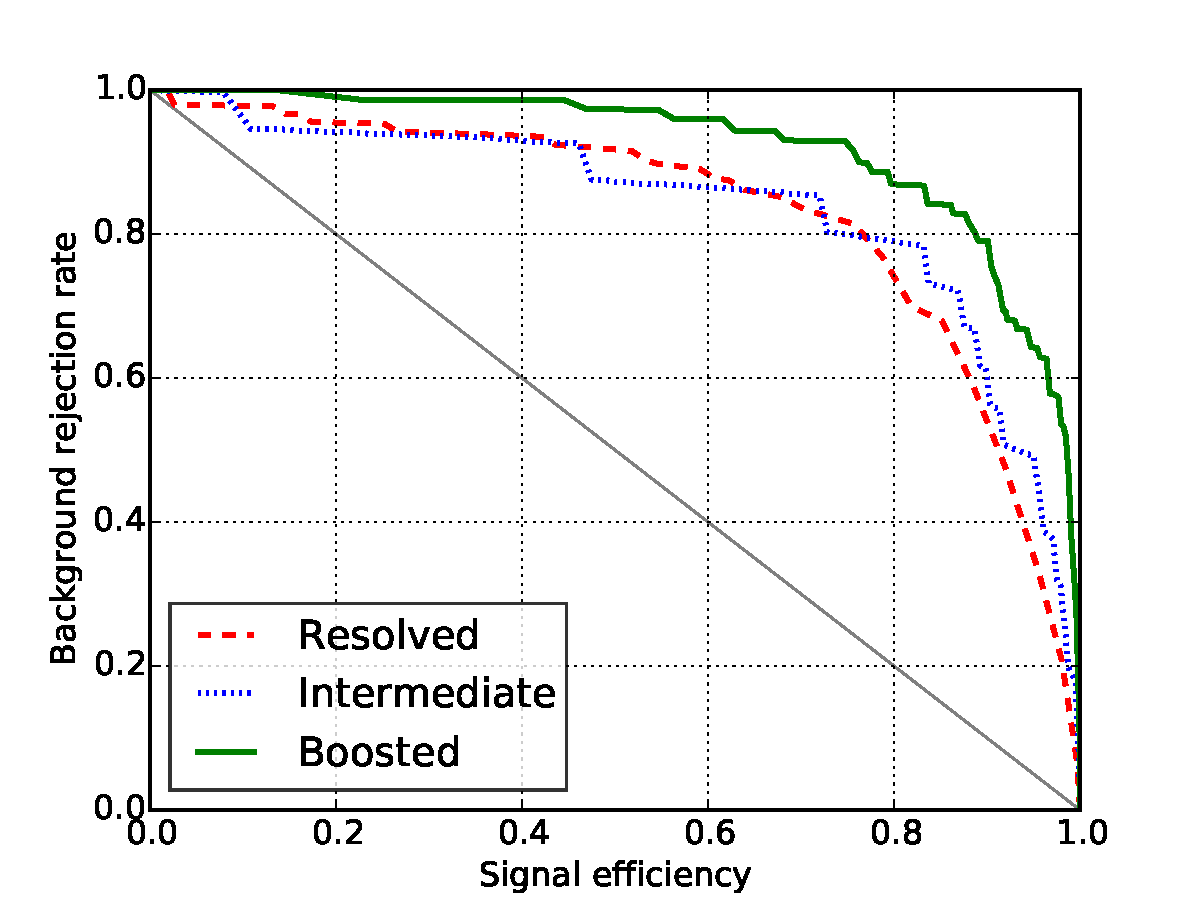
\includegraphics[width=0.65\textwidth]{plots/roc.pdf}
\caption{\small ROC curve for the background rejection rate as a function of the signal
  selection efficiency as the cut in the ANN output is varied.
  %
  We show the results for the three exclusive categories: boosted, intermediate
  and resolved.
}
\label{fig:exampleroc}
\end{center}
\end{figure}
%%%%%%%%%%%%%%%%%%%%%%%%%%%%%%%%%%%%%

From Fig.~\ref{fig:exampleroc} we see that, always starting from the signal
and background events that survive the basic cut-based analysis,
one can achieve a  signal
efficiency of $\sim 80\%$ while reducing the background by
$60\%$, $55\%$ and $45\%$ in the boosted, intermediate and resolved
categories respectively.
%
It is easy to translate these factors into an  improvement factor of the pre-MVA
signal significance $S/\sqrt{B}$.
%
For example, requiring a signal efficiency of 90\%, we find a background rejection
rate of $40\%$, $30\%$ and $20\%$ respectively, which corresponds to an increase
in $S/\sqrt{B}$ of 1.2, 1.1 and 1.0 respectively.

Of course, and important restriction on the range of allowed cuts in the ANN output
is that the cut cannot be so hard that the actual number of signal events expected
at the HL-LHC becomes unreasonably small.
%
To verify how many signal and background events are left after the MVA cut,
we show in Fig.~\ref{fig:nev2} the number of signal (dashed lines) and background (solid lines)
  events expected at the HL-LHC as a function of the cut in the ANN output,
  for the three separate categories.
  %
  Note that the value of the cut in the ANN cut can be separately optimised in the three
  categories, even if here we plot them together for easiness of presentation.

%%%%%%%%%%%%%%%%%%%%%%%%%%%%%%%%%%%%%%%%%%%%%%
\begin{figure}[t]
\begin{center}
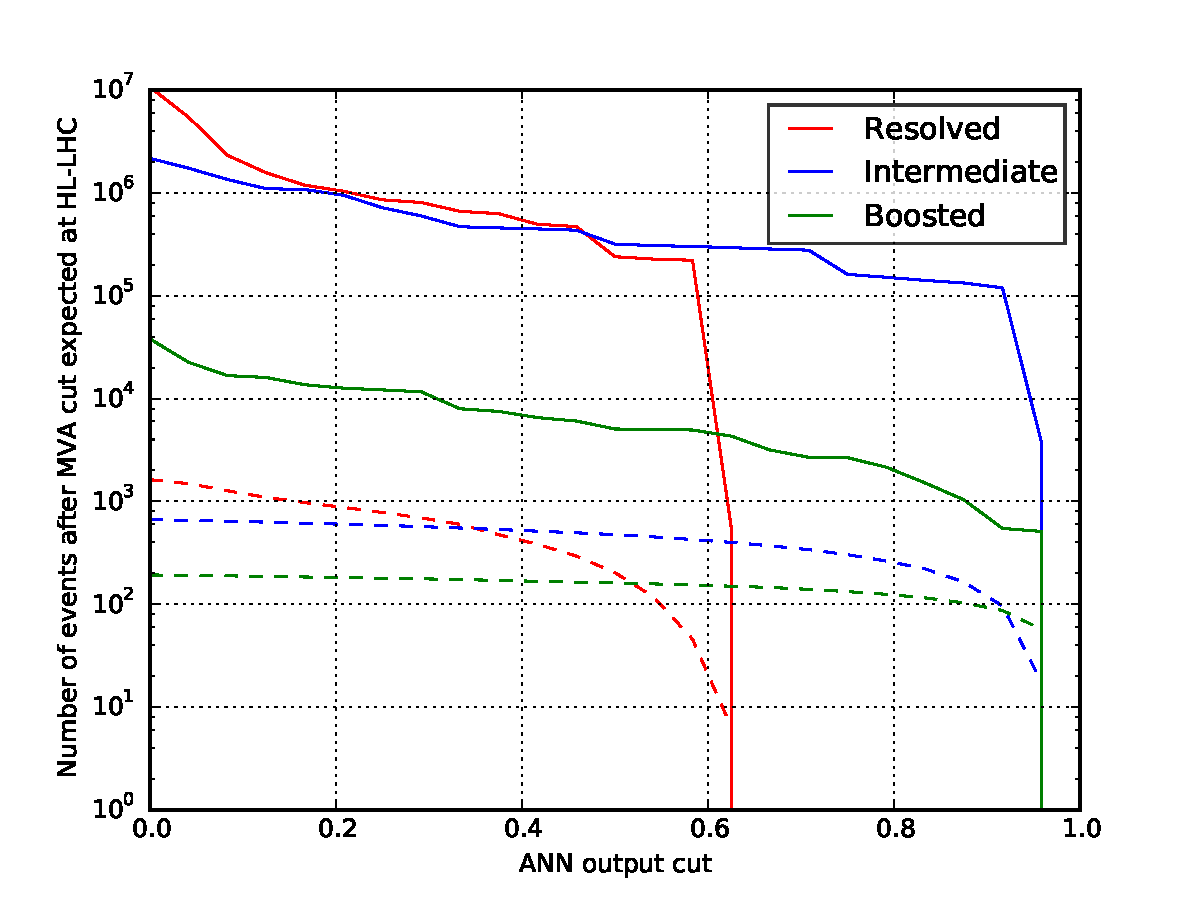
\includegraphics[width=0.65\textwidth]{plots/nev2.pdf}
\caption{\small Number of signal (dashed lines) and background (solid lines)
  events expected at the HL-LHC as a function of the cut in the ANN output,
  for the three separate categories.
}
\label{fig:nev2}
\end{center}
\end{figure}
%%%%%%%%%%%%%%%%%%%%%%%%%%%%%%%%%%%%%

As can be seen from Fig.~\ref{fig:nev2}, in the boosted category
event with a cut in the ANN output as hard as 0.9 we are still left
with around 100 events at the HL-LHC, which is a reasonable number,
which the background being reduced substantially to around
500 events.
%
A similar cut would work fine for the intermediate category, though here
the backgrounds are much larger and thus the expected signal significance smaller.
%
For the resolved case, the signal significance would be only slightly
improved for any value of the cut.

A very useful property of MVA's such as the one used in this work
is that they provide direct  physical insight about which of the
input variables contribute the most to the signal over background
separation.
%
In the case of ANNs, this can be quantified by computing the sum
of the absolute value of al the weights connected to a given
input neuron $i$, that is
\be
\label{eq:totweight}
\omega^{\rm tot}_i \equiv \sum_{k=1}^5 \Big|\omega^{(2)}_{ki}\Big| \, ,
\qquad i=1,\ldots,N_{\rm var} \, ,
\ee
with $\omega^{(2)}_{ki}$ the value of the weight connecting
the $k$-th neutron of the second layer with the $i$-th neuron of
the first (input) layer.
%
The input variables with a larger value of $\omega^{\rm tot}_i$ will those
be the ones that play a dominant role in enhancing the signal
discrimination using the MVA.

%
In Fig.~\ref{fig:nnweights} we show
the distribution of the total associated weight,
Eq.~(\ref{eq:totweight}) for each of the $N_{\rm var}$ input
variables of the resolved (left plot) and boosted (right plot) categories.
%
The notation for the various kinematic variables is the same
as in Sect.~\ref{sec:input}.
%
The scale of the $y$ axis is arbitrary, and the important information
is contained in the relative strengths of the total associated weight
for each of the input variables.



%%%%%%%%%%%%%%%%%%%%%%%%
\begin{figure}[t]
\begin{center}
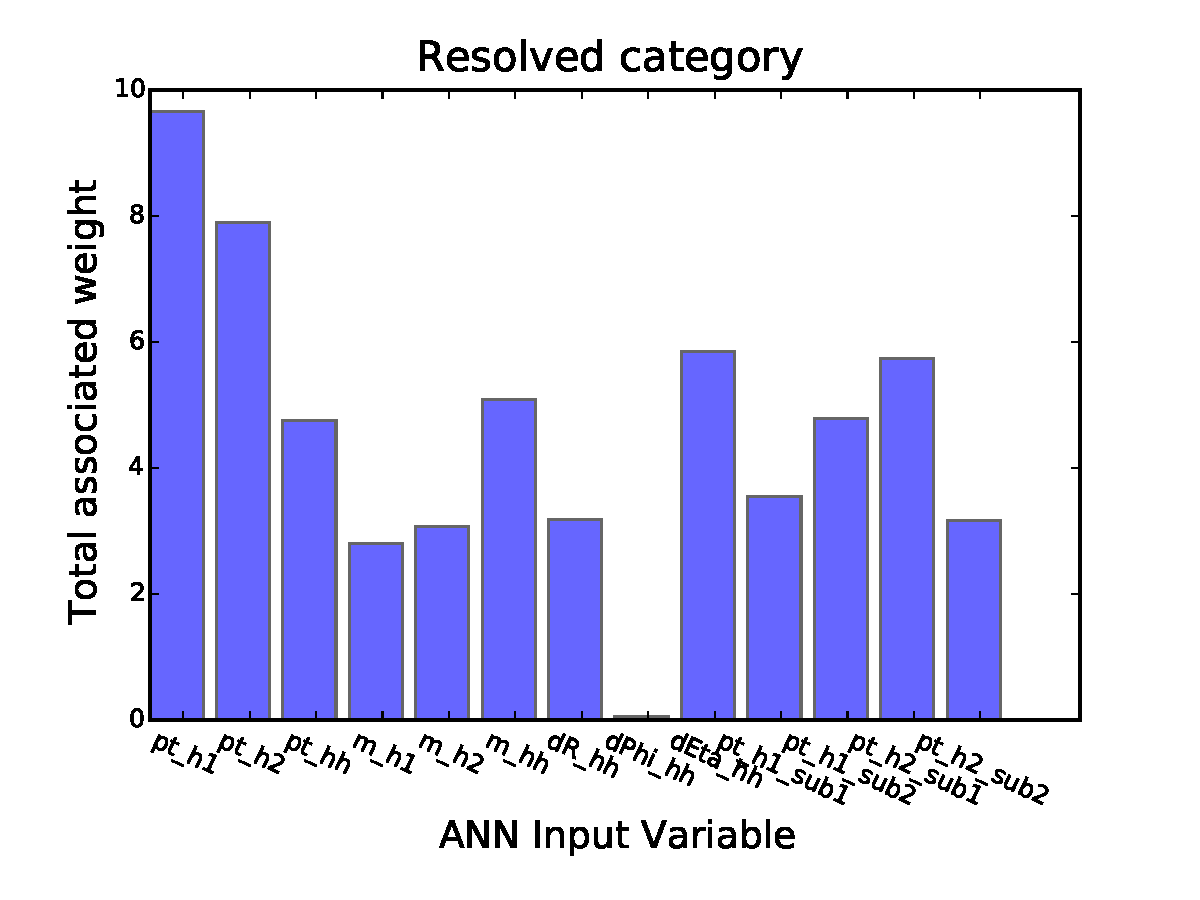
\includegraphics[width=0.48\textwidth]{plots/res_wgthist.pdf}
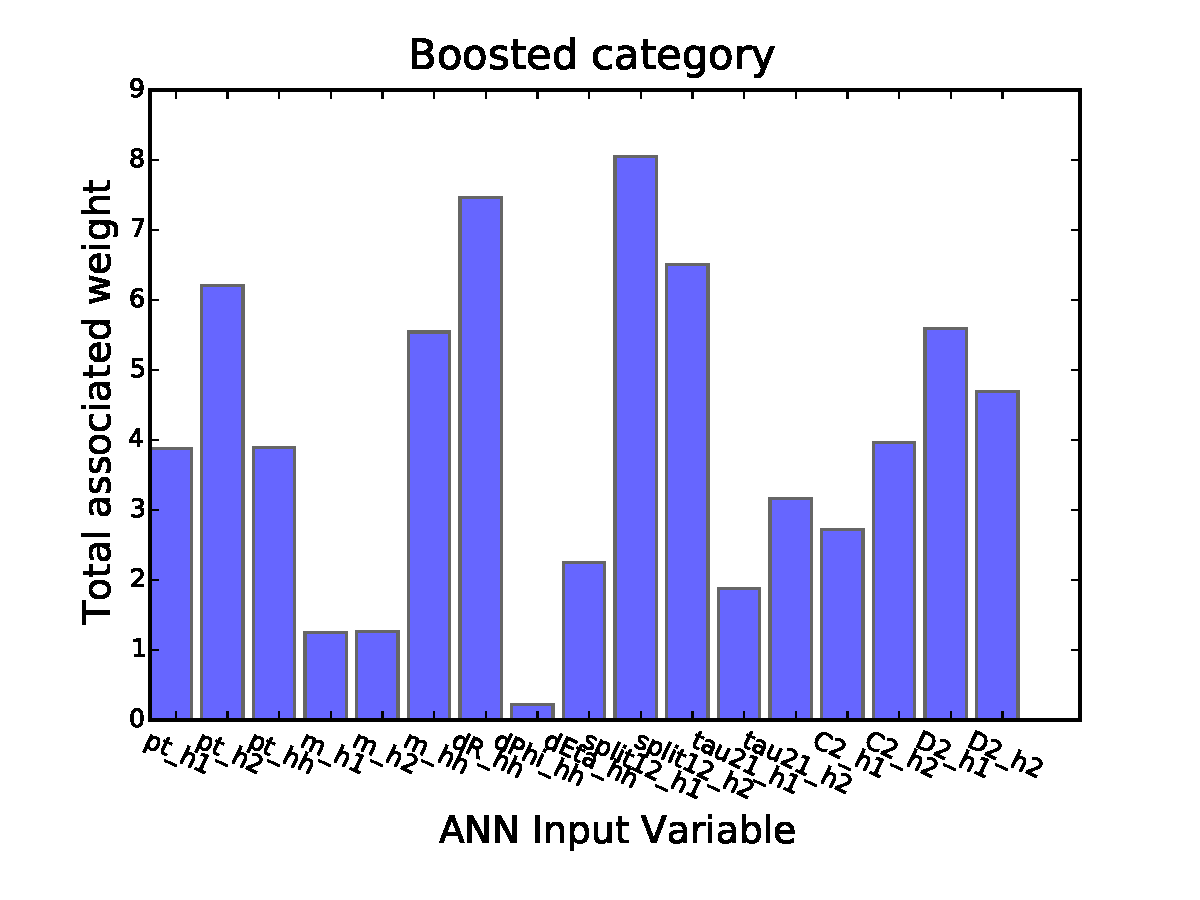
\includegraphics[width=0.48\textwidth]{plots/boosted_wgthist.pdf}
\caption{\small
Distribution of the total associated weight,
Eq.~(\ref{eq:totweight}) for each of the $N_{\rm var}$ input
variables of the resolved (left plot) and boosted (right plot) categories.
%
See Sect.~\ref{sec:input} for a description of each of the input
variables to the MVA in the two cases.
}
\label{fig:nnweights}
\end{center}
\end{figure}
%%%%%%%%%%%%%%%%%%%%%%%

The results of Fig.~\ref{fig:nnweights} clearly illustrate which variables
are more discriminative between the signal and the background.
%
Let's begin discussing the resolved analysis.
%
In this category, the variables that lead to
a higher discrimination power
are the $p_T$ of the two reconstructed Higgs, and then on a similar
footing other variables like the $p_T$ of the individual jets
and the mass of the di-Higgs system.
%
The only variable which seems to contain to information at all
is the $\Delta \phi_{hh}$ separation between the two
Higgs candidates.


For the boosted category, we see that substructure variables
are the most helpful ones, in particular the $k_t$ splitting scales
$\sqrt{d_{12}}$ and the subjetiness ratio $\tau_{12}$.
%
The ratio of energy correlations $D_2$ and $C_2$ also help,
in particular the former.
%
From the more traditional variables, the angular
separation between the two large-$R$ jets $\Delta R_{hh}$,
the invariant mass of the di-Higgs system $m_{hh}$ and the various
$p_T$ also have discrimination power.
%
Other variables provide limited information, in particular the invariant
mass of the Higgs candidates, $m_{h_1}$ and $m_{h_2}$, due to the realistic
simulation of detector resolution introduced with the smearing.
%
We have verified that signal significance in the boosted category is substantially
degraded if substructure variables are not used, emphasizing that
in the boosted category jet substructure provides the best handle
to separate signal and background.

At this point we have all the ingredients that we need to determine the optimal
value of the MVA output cut and quantify the final values of the signal
significance $S/\sqrt{B}$ and $S/B$ in our three categories.
%
These optimal values are determining by the maximisation of $S/\sqrt{B}$,
ensuring that the number of events which is left at the HL-LHC is large
enough, and also that the actual number of MC events used for the ANN training
is still large enough to avoid the biases of a small training sample.
%
The post-MVA results for $S/\sqrt{B}$ and $S/B$ as a function of the cut
in the ANN output for each of the three categories are shown in
Fig.~\ref{fig:sb_mva}.
%
As mentioned before, the optimal cuts are determined independently for each
category.
%
Note that the values of $S/\sqrt{B}$ and $S/B$ in the three cases should correspond
to the same values at the end of the cut-based analysis, as
can be verified by looking at the {\bf C2} row of Table~\ref{table:cutflow}.
%
Indeed, at the end of the cut based analysis $S/\sqrt{B}$ is approximately
1.0, 0.5 and 0.5 for the boosted, intermediate and resolved
categories, as can be seen from Fig.~\ref{fig:sb_mva}.

%%%%%%%%%%%%%%%%%%%%%%%%
\begin{figure}[t]
\begin{center}
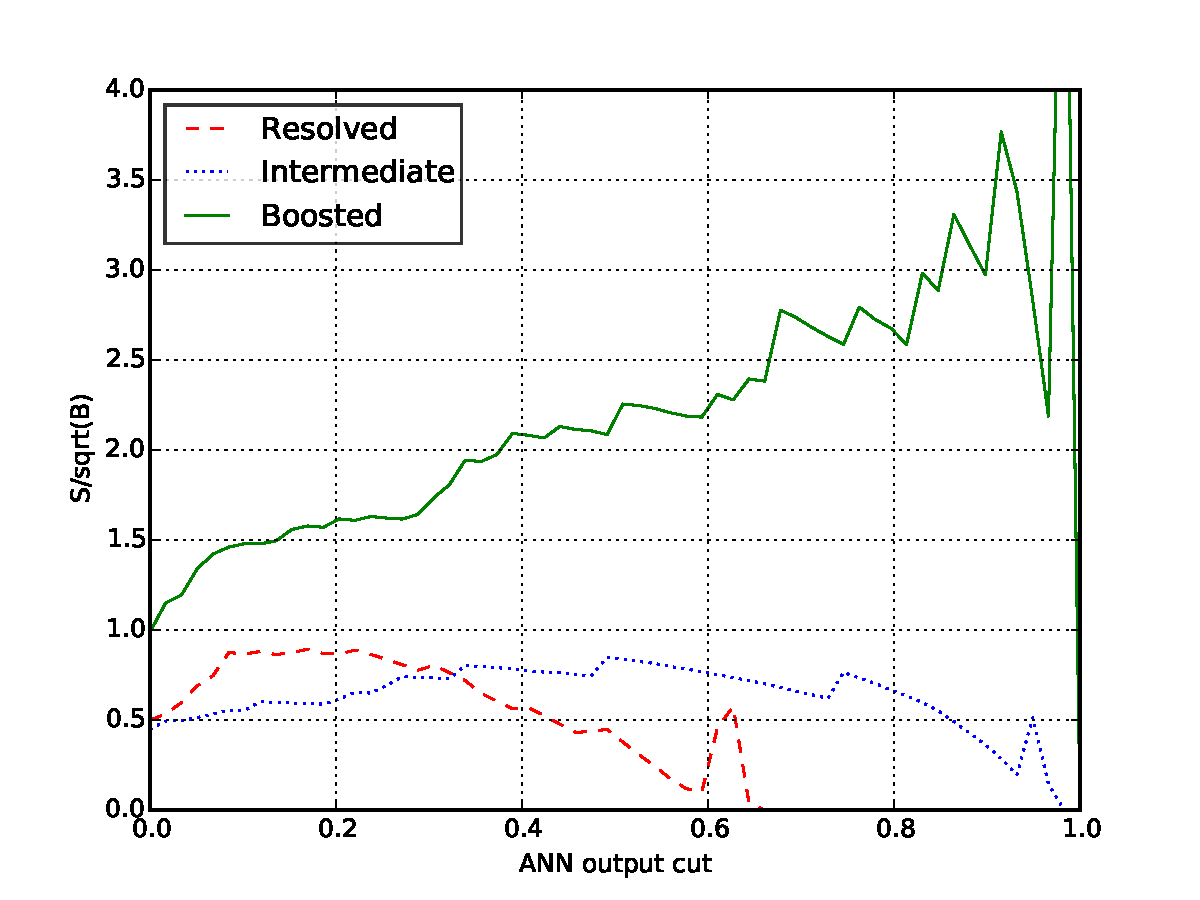
\includegraphics[width=0.48\textwidth]{plots/ssb.pdf}
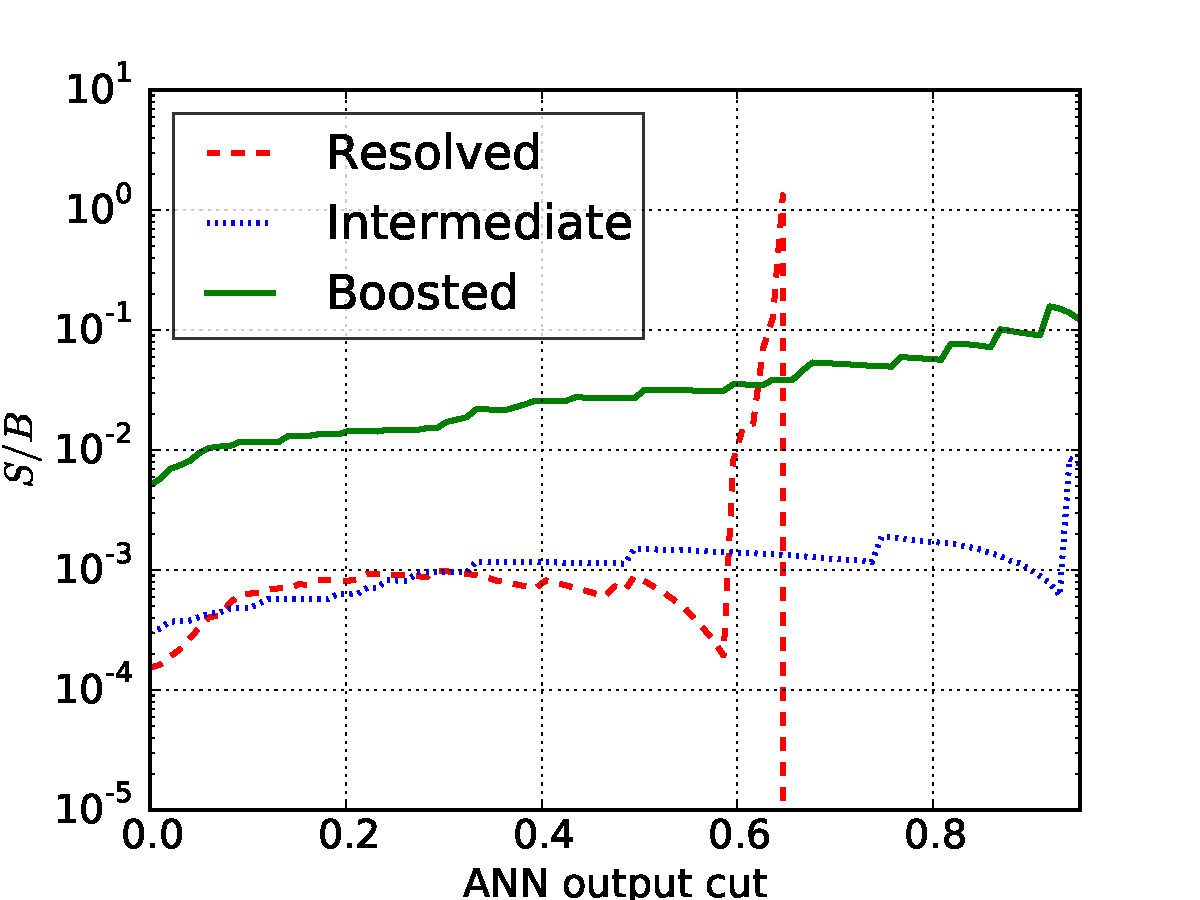
\includegraphics[width=0.48\textwidth]{plots/sb.pdf}
\caption{\small
  The values of the signal significance $S/\sqrt{B}$ and of the
  signal over background ratio $S/B$ for the boosted, intermediate
  and resolved categories.
  %
  Note that the optimal cuts are determined independently for each
  category.
  %
  The no-cut values correspond to the  cut-based analysis
  results from Table~\ref{table:cutflow}.
}
\label{fig:sb_mva}
\end{center}
\end{figure}
%%%%%%%%%%%%%%%%%%%%%%%

The results of Fig.~\ref{fig:sb_mva} are interesting in that they show
that for the resolved and boosted categories the improvement in signal
significance arising from the MVA is rather moderate, less that a factor two
in the two cases.
%
For no value of the cut the $S/\sqrt{B}$ value in these two categories
goes above one.
%
The real usefulness of the MVA can be seen for the resolved category,
where the signal significance rises from around 1.0 in the cut-based
analysis to above 3.0 for values of the ANN output cut above 0.85.
%
This value of the cut seems reasonable, since we know from Fig.~\ref{fig:nev2}
that the number of signal events at the HL-LHC is still quite substantial,
of the order of 100.
%
Therefore, thanks to the MVA, we predict that one should be able
to find evidence for the production of Higgs boson pairs
at the HL-LHC using the $4b$ channel alone.

Another very important benefit of the MVA applied to the boosted
category is that fact that the background is substantially
reduced so that $S/B$ can be as large as 10\% for the optimal
values of the ANN output cut.
%
Note that this is not true for the other two categories,
where $S/B$ is roughly constant.
%
A reasonably large value of $S/B$ is extremely beneficial
from the experimental point of view, since it indicates
that the measurement is feasible even if the
systematic uncertainties are not very small.

Our final results are summarized in Table~\ref{table:cutflowMVA}, where we indicate
the value of the optimal cut in each category,
the number of signal and background events $N_{\rm ev}$,
and also $S/\sqrt{B}$ and $S/B$.
%
For completeness, we also include the results after the cut-based
analysis.
%
Given that the signal significance is much larger in the boosted as
compared to the other two categories, no additional information
could be obtained by combining the significance of the three
categories, and it seems more efficient to perform
the analysis exclusively in the boosted category.


%%%%%%%%%%%%%%%%%%%%%%%%%%%%%%%%%%%%%%%%%%%%%%%%%%%%%
\begin{table}[t]
  \centering
  \begin{tabular}{c|c|c|c||c|c|c|c}
    \hline
    \multicolumn{8}{c}{Boosted category}\\
    \hline
    \hline
    \multicolumn{4}{c||}{no MVA cut} & \multicolumn{4}{c}{optimal MVA cut}\\
    \multicolumn{4}{c||}{$y_{\rm mva}=0$} & \multicolumn{4}{c}{$y_{\rm mva}=0.85$}\\
    \hline
    \multicolumn{2}{c|}{$N_{\rm ev}$} &  $S/\sqrt{B}$  & $S/B$
    & \multicolumn{2}{c|}{$N_{\rm ev}$} &  $S/\sqrt{B}$  & $S/B$\\
        Signal & Back   &     &   &  Signal & Back   &     &    \\
    \hline
      193   &  $3.8\,10^4$    &  0.99    &  $5.1\,10^{-3}$  &  &  &  & \\
        \hline
  \end{tabular}
   $\,$\\
  \vspace{0.4cm}
  \noindent
  \begin{tabular}{c|c|c|c||c|c|c|c}
    \hline
    \multicolumn{8}{c}{Intermediate category}\\
    \hline
    \hline
    \multicolumn{4}{c||}{no MVA cut} & \multicolumn{4}{c}{optimal MVA cut}\\
    \multicolumn{4}{c||}{$y_{\rm mva}=0$} & \multicolumn{4}{c}{$y_{\rm mva}=0.85$}\\
    \hline
    \multicolumn{2}{c|}{$N_{\rm ev}$} &  $S/\sqrt{B}$  & $S/B$
    & \multicolumn{2}{c|}{$N_{\rm ev}$} &  $S/\sqrt{B}$  & $S/B$\\
        Signal & Back   &     &   &  Signal & Back   &     &    \\
    \hline
      660   &   $2.2\,10^6$   &   0.45   &  $3.1\,10^{-4}$ &  &  &  & \\
        \hline
  \end{tabular}
    $\,$\\
  \vspace{0.4cm}
  \noindent
  \begin{tabular}{c|c|c|c||c|c|c|c}
    \hline
    \multicolumn{8}{c}{Resolved category}\\
    \hline
    \hline
    \multicolumn{4}{c||}{no MVA cut} & \multicolumn{4}{c}{optimal MVA cut}\\
    \multicolumn{4}{c||}{$y_{\rm mva}=0$} & \multicolumn{4}{c}{$y_{\rm mva}=0.85$}\\
    \hline
    \multicolumn{2}{c|}{$N_{\rm ev}$} &  $S/\sqrt{B}$  & $S/B$
    & \multicolumn{2}{c|}{$N_{\rm ev}$} &  $S/\sqrt{B}$  & $S/B$\\
        Signal & Back   &     &   &  Signal & Back   &     &    \\
    \hline
      $1.6\,10^{3}$   &   $1.1\,10^{7}$   & 0.50     &  $1.5\,10^{-4}$   &  &  &  & \\
        \hline
  \end{tabular}
  \caption{\small The results for the number of signal and
    background events
    at the HL-LHC for both the cut-based analysis and after the
    optimal MVA cut, as well as the $S/\sqrt{B}$ and $S/B$
    values in the two cases.
    %
    From top to bottom we show the results for boosted,
    intermediate and resolved categories.
    %
    Note that the optimal value of the MVA cut
    is different in each of the three categories.
    \label{table:cutflowMVA}
  }
\end{table}
%%%%%%%%%%%%%%%%%%%%%%%%%%%%%%%%%%%%%%%%%%%%%%%%%%%%%




\subsection{Another look at jet substructure variables}

It is now worth trying to understand where does the increase in signal significance
achieved after the MVA comes from.
%
As we will show now, the MVA has correctly identified which of the substructure
variables are more discriminant between signal and background distributions,
and combined this information to determine an optimal cut to maximize signal
significance.

For instance, in the boosted category, the analyses of the
size of the neural network weights clearly indicates that the subjetiness
$\tau_{12}$ and the energy correlations $C_2$ are two of the most useful
variables.
%
To verify that indeed these two variables are quite different between signal
and background events, in Fig.~\ref{fig:mva_substructure_1}
we show the subjetiness $\tau_{12}$ and the energy correlation between
signal and background.
%
We indeed verify that the two shapes are quite different,
reflecting the differences in the internal structure of jets
between QCD jets and jets originated from the Higgs decays.


%%%%%%%%%%%%%%%%%%%%%%%%%%%%
\begin{figure}[t]
\begin{center}
  \includegraphics[width=0.48\textwidth]{plots/tau21_h0_res_C1_boost.pdf}
  \includegraphics[width=0.48\textwidth]{plots/EEC_C2_h0_res_C1_boost.pdf}
  \caption{\small Left plot: subjetiness.
    Right plot: energy correlations.
}
\label{fig:mva_substructure_1}
\end{center}
\end{figure}
%%%%%%%%%%%%%%%%%%%%%%%


